\documentclass{beamer}
\usetheme[white]{Wisconsin}
\usepackage{longtable}
\usepackage{listings}
\usepackage{color}
%% The amssymb package provides various useful mathematical symbols
\usepackage{amssymb}
%% The amsthm package provides extended theorem environments
\usepackage{amsthm} \usepackage{amsmath} \usepackage{tmadd,tmath}
\usepackage[mathcal]{euscript} \usepackage{color}
\usepackage{textcomp}
\usepackage{algorithm,algorithmic}
\definecolor{listinggray}{gray}{0.9}
\definecolor{lbcolor}{rgb}{0.9,0.9,0.9}
\lstset{
  backgroundcolor=\color{lbcolor},
  tabsize=4,
  rulecolor=,
  language=c++,
  basicstyle=\scriptsize,
  upquote=true,
  aboveskip={1.5\baselineskip},
  columns=fixed,
  showstringspaces=false,
  extendedchars=true,
  breaklines=true,
  prebreak =
  \raisebox{0ex}[0ex][0ex]{\ensuremath{\hookleftarrow}},
  frame=single,
  showtabs=false,
  showspaces=false,
  showstringspaces=false,
  identifierstyle=\ttfamily,
  keywordstyle=\color[rgb]{0,0,1},
  commentstyle=\color[rgb]{0.133,0.545,0.133},
  stringstyle=\color[rgb]{0.627,0.126,0.941},
}

%% colors
\setbeamercolor{boxheadcolor}{fg=white,bg=UWRed}
\setbeamercolor{boxbodycolor}{fg=black,bg=white}


%%---------------------------------------------------------------------------%%
\author{\small Stuart R. Slattery and Paul P.H. Wilson, University of Wisconsin - Madison
  \\ \
  \\ Thomas M. Evans, Oak Ridge National Laboratory
}

\date{\today} 
\title{A Spectral Analysis of the Domain Decomposed Monte Carlo Method
for Linear Systems}
\begin{document}
\maketitle

%%---------------------------------------------------------------------------%%
\begin{frame}{Motivation}

  \begin{itemize}
  \item First proposed by J. Von Neumann and S.M. Ulam in the 1940's
    \bigskip
  \item General lack of published work
    \bigskip
  \item Recent work by Evans and others has yielded new potential
    applications
    \bigskip
  \item Implications for resilient exascale solver strategies
    \bigskip
  \item Domain decomposed parallelism has yet to be exploited - would
    like a preliminary analytic framework
  \end{itemize}

\end{frame}

%%---------------------------------------------------------------------------%%
\begin{frame}{Monte Carlo Linear Solver Preliminaries}

  \begin{itemize}
  \item Split the linear operator
  \end{itemize}

  \[
  \ve{H} = \ve{I} - \ve{A}
  \]

  \[
  \ve{A}\ve{x} = \ve{b} \ \ \ \rightarrow \ \ \ \ve{x} = \ve{H} \ve{x}
  + \ve{b}
  \]

  \medskip
  \begin{itemize}
  \item Generate the \textit{Neumann series}
  \end{itemize}
  
  \[
  \ve{A}^{-1} = (\ve{I}-\ve{H})^{-1} = \sum_{k=0}^{\infty} \ve{H}^k
  \]

  \medskip
  \begin{itemize}
  \item Require $\rho(\ve{H}) < 1$ for convergence
  \end{itemize}

  \[
  \ve{A}^{-1}\ve{b} = \sum_{k=0}^{\infty} \ve{H}^k\ve{b} = \ve{x}
  \]

\end{frame}

%%---------------------------------------------------------------------------%%
\begin{frame}{Monte Carlo Linear Solver Preliminaries}

  \begin{itemize}
  \item Expand the Neumann series
  \end{itemize}

  \[
  x_i = \sum_{k=0}^{\infty}\sum_{i_1}^{N}\sum_{i_2}^{N}\ldots
  \sum_{i_k}^{N}h_{i,i_1}h_{i_1,i_2}\ldots h_{i_{k-1},i_k}b_{i_k}
  \]

  \begin{itemize}
  \item Define a sequence of state transitions
  \end{itemize}
  
  \[
  \nu = i \rightarrow i_1 \rightarrow \cdots \rightarrow i_{k-1}
  \rightarrow i_{k}
  \]

  \begin{itemize}
  \item Use the adjoint Neumann-Ulam decomposition\footnote{The
    Hadamard product $\ve{A} = \ve{B} \circ \ve{C}$ is defined
    element-wise as $a_{ij} = b_{ij} c_{ij}$.}
  \end{itemize}

  \[
  \ve{H}^{T} = \ve{P} \circ \ve{W}
  \]

  \[
  p_{ij} = \frac{|h_{ji}|}{\sum_j |h_{ji}|},\ w_{ij} =
  \frac{h_{ji}}{p_{ij}}
  \]

\end{frame}

%%---------------------------------------------------------------------------%%
\begin{frame}{Adjoint Method}

  \medskip
  \begin{itemize}
  \item Build the estimator and expectation value
  \end{itemize}

  \[
  X_j(\nu) = \sum_{m=0}^k W_{m} \delta_{i_m,j}
  \]

  \[
  \begin{split}
    E\{X_j\} &= \sum_{\nu}P_{\nu}X_{\nu} =
    \sum_{k=0}^{\infty}\sum_{i_1}^{N}\sum_{i_2}^{N}\ldots
    \sum_{i_k}^{N} b_{i_0} h_{i_0,i_1}h_{i_1,i_2}\ldots
    h_{i_{k-1},i_k} \delta_{i_k,j} \\ &= x_{j}
  \end{split}
  \]

  \medskip
  \begin{itemize}
  \item Terminate a random walk below a weight cutoff, $W_m < W_c$
  \end{itemize}

\end{frame}

%%---------------------------------------------------------------------------%%
\begin{frame}{Adjoint Method: Evolution of a Solution}

  \begin{figure}[h!]
    \begin{center}
      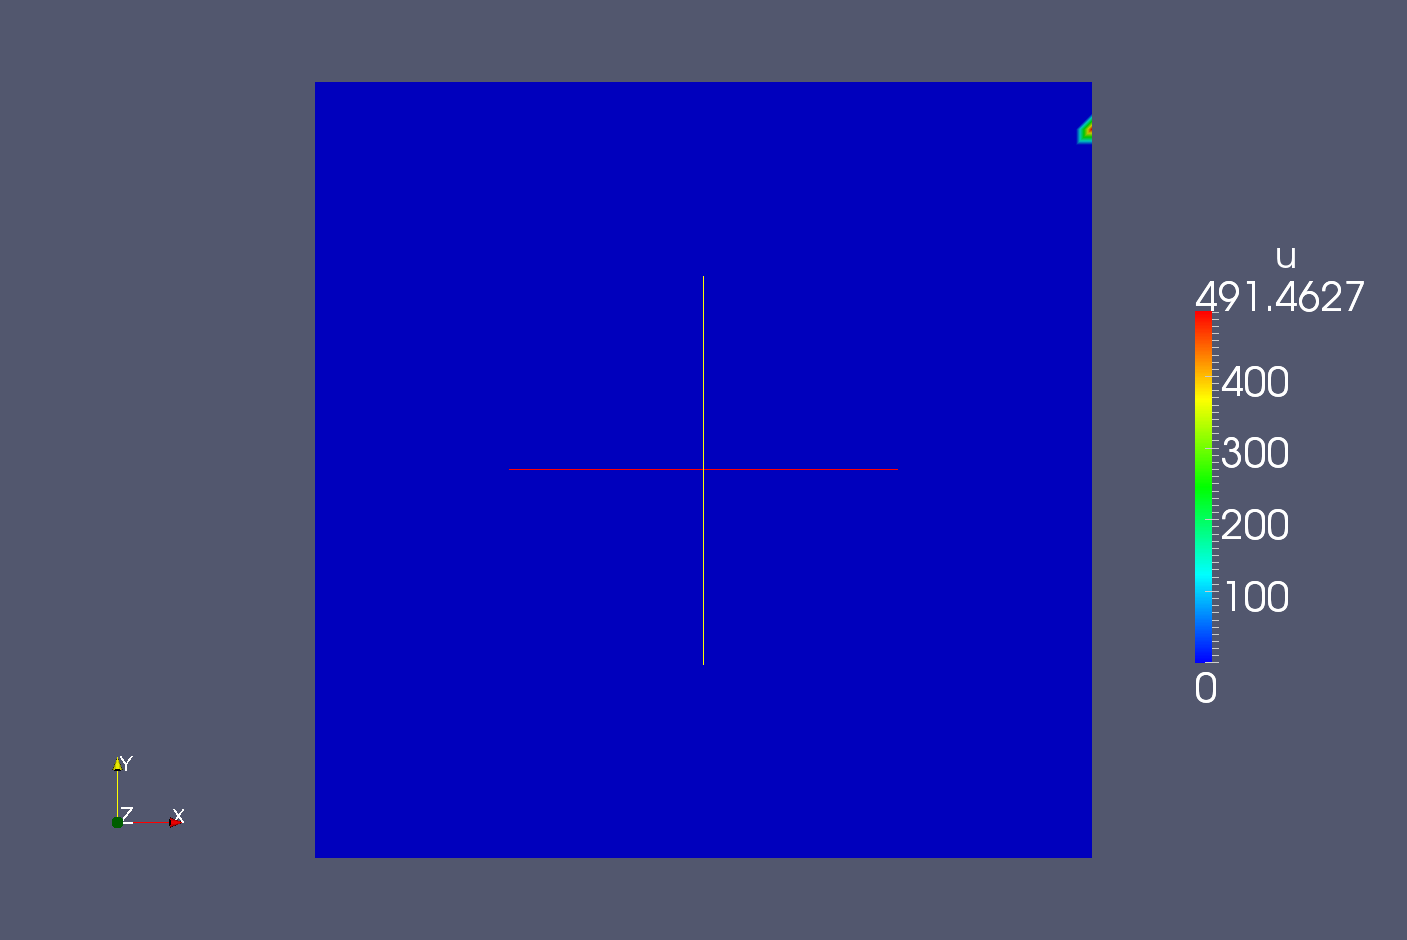
\includegraphics[width=4in]{adjoint_1.png}
    \end{center}
    \caption{\textbf{Adjoint solution to Poisson Equation.}
      \textit{\sn{1}{0} total histories, 0.286 seconds CPU time.} }
  \end{figure}

\end{frame}

%%---------------------------------------------------------------------------%%
\begin{frame}{Adjoint Method: Evolution of a Solution}

  \begin{figure}[h!]
    \begin{center}
      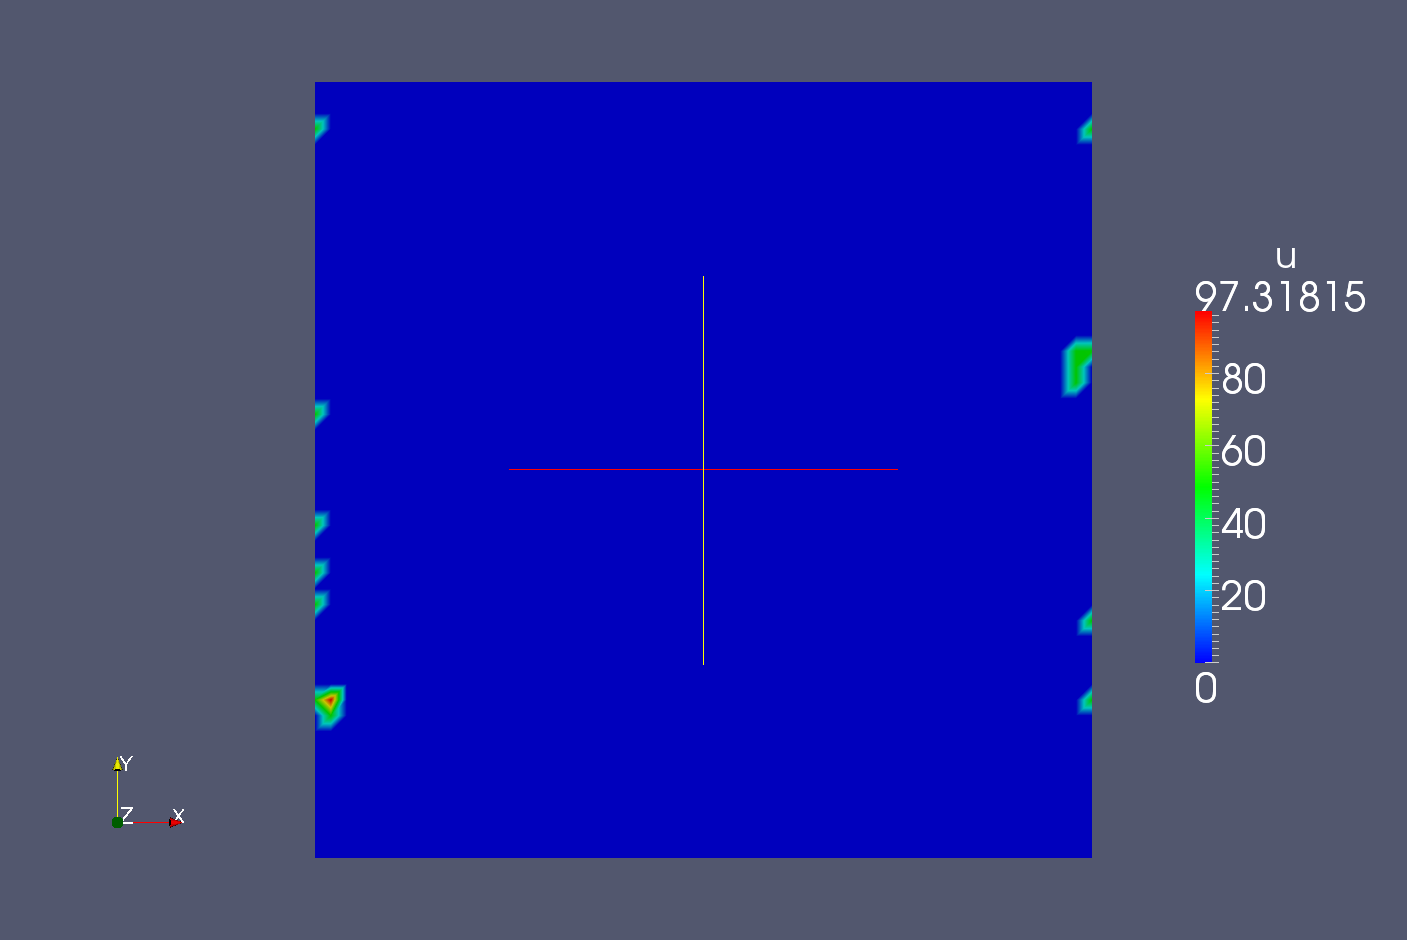
\includegraphics[width=4in]{adjoint_10.png}
    \end{center}
    \caption{\textbf{Adjoint solution to Poisson Equation.}
      \textit{\sn{1}{1} total histories, 0.278 seconds CPU time.} }
  \end{figure}

\end{frame}

%%---------------------------------------------------------------------------%%
\begin{frame}{Adjoint Method: Evolution of a Solution}

  \begin{figure}[h!]
    \begin{center}
      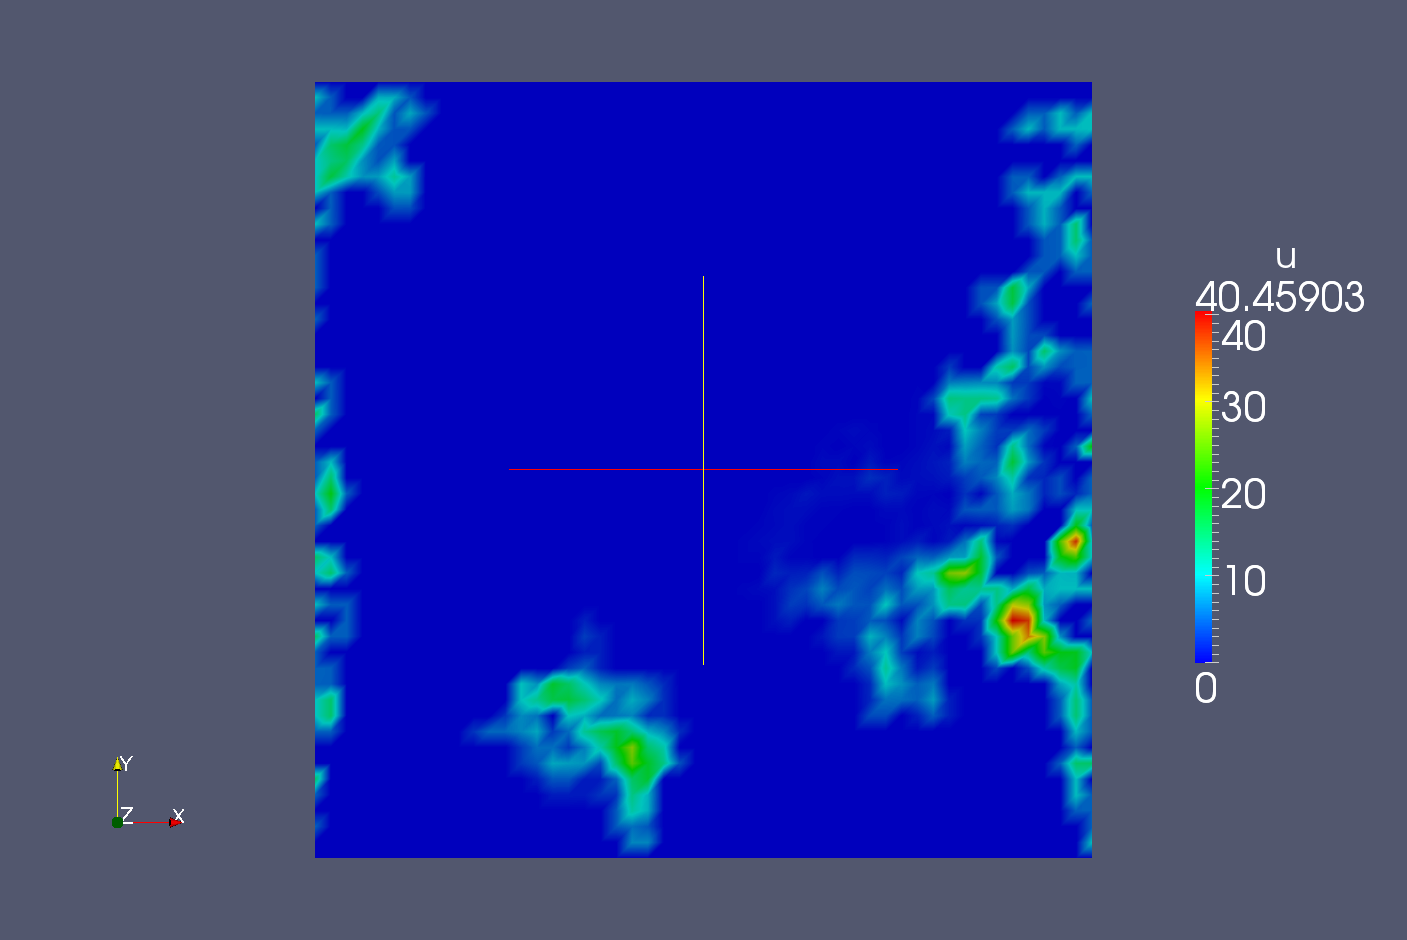
\includegraphics[width=4in]{adjoint_100.png}
    \end{center}
    \caption{\textbf{Adjoint solution to Poisson Equation.}
      \textit{\sn{1}{2} total histories, 0.275 seconds CPU time.} }
  \end{figure}

\end{frame}

%%---------------------------------------------------------------------------%%
\begin{frame}{Adjoint Method: Evolution of a Solution}

  \begin{figure}[h!]
    \begin{center}
      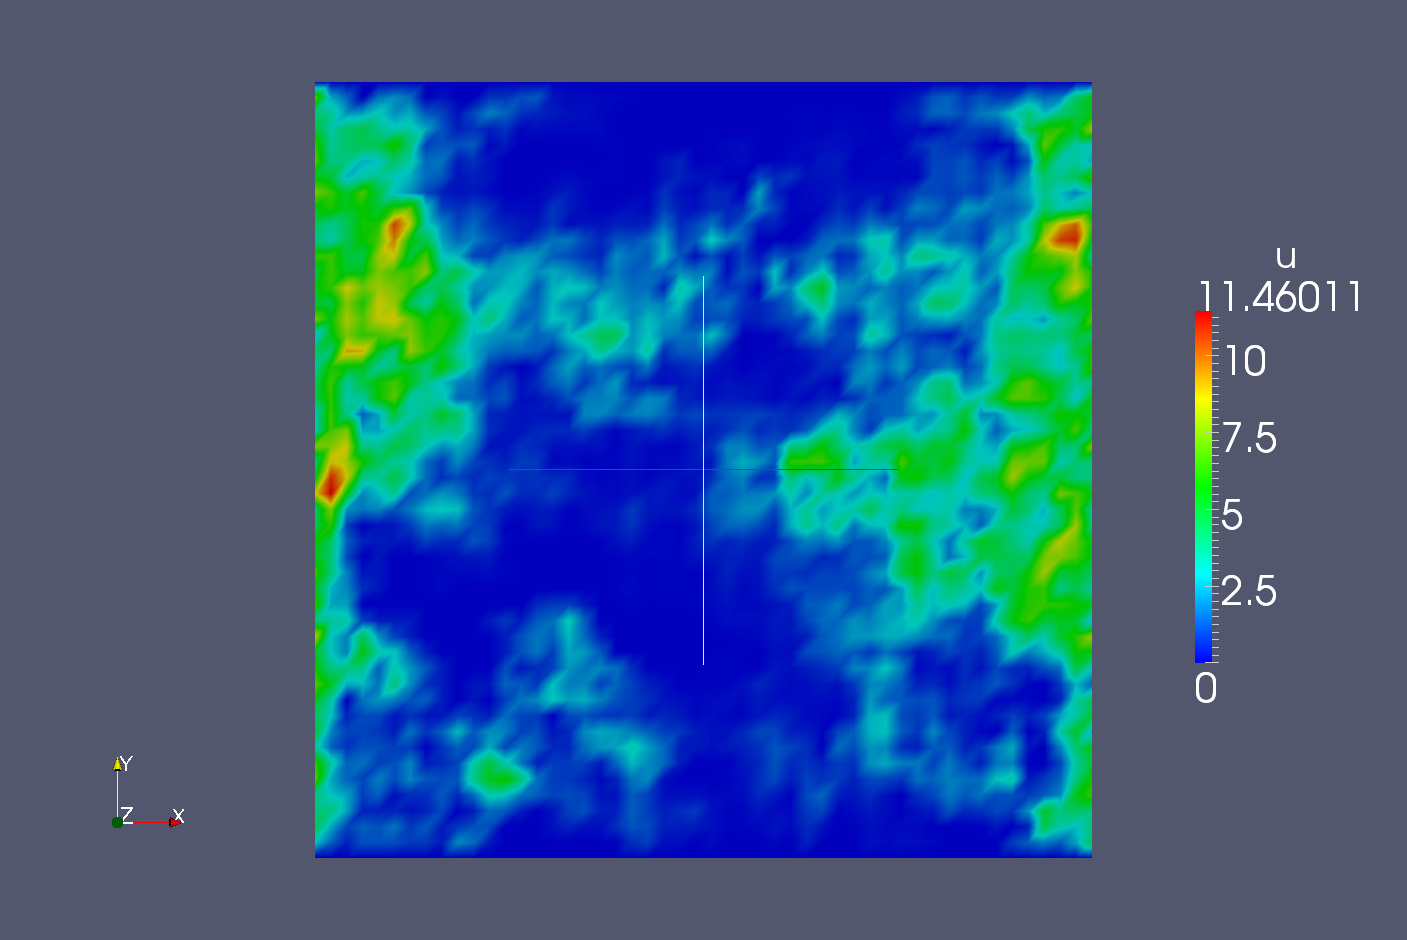
\includegraphics[width=4in]{adjoint_1000.png}
    \end{center}
    \caption{\textbf{Adjoint solution to Poisson Equation.}
      \textit{\sn{1}{3} total histories, 0.291 seconds CPU time.} }
  \end{figure}

\end{frame}

%%---------------------------------------------------------------------------%%
\begin{frame}{Adjoint Method: Evolution of a Solution}

  \begin{figure}[h!]
    \begin{center}
      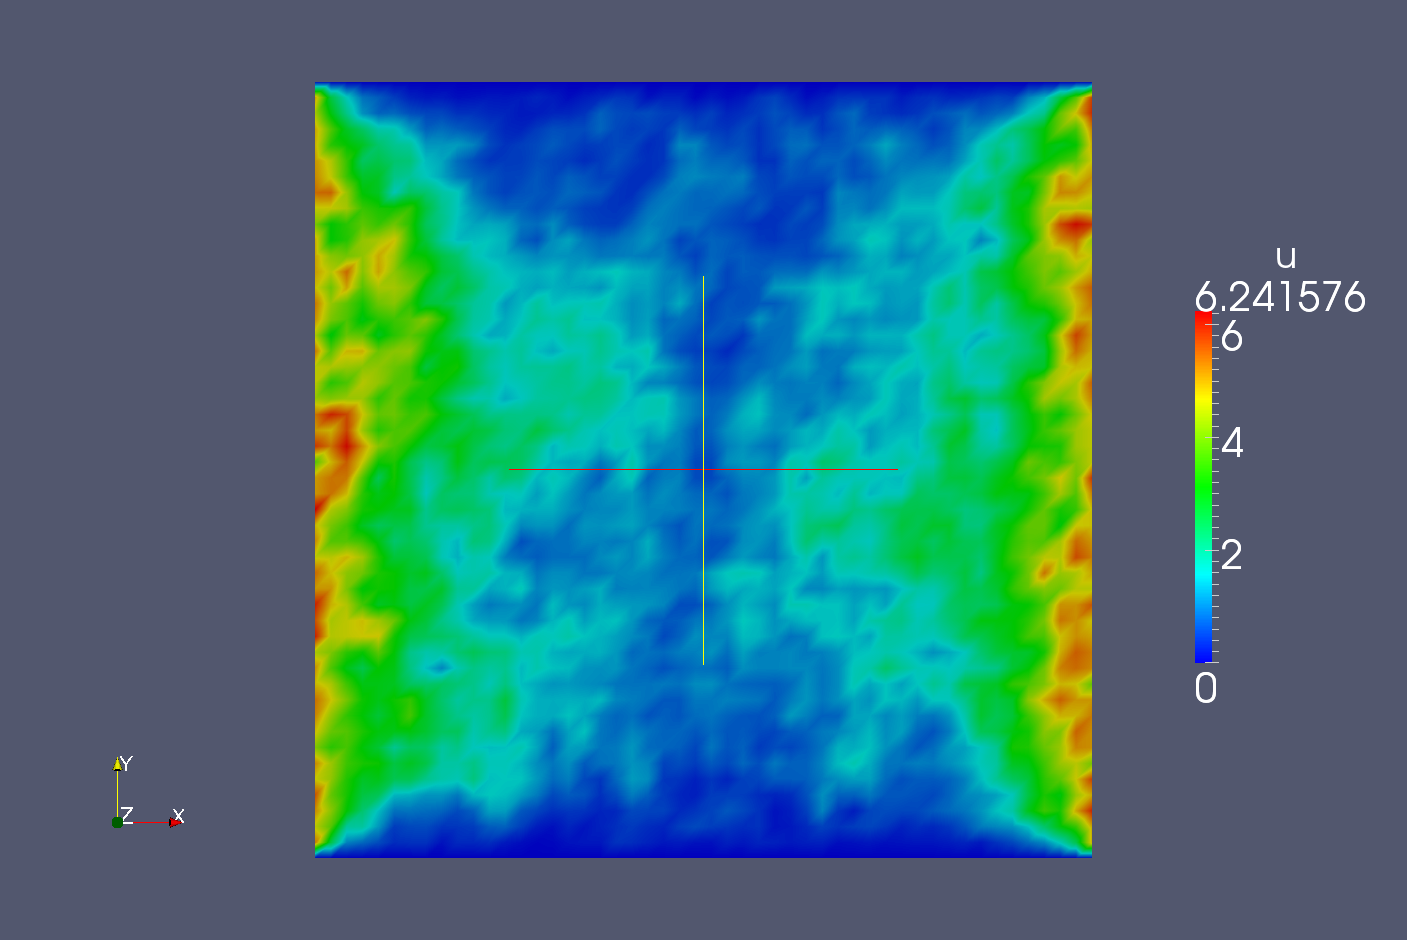
\includegraphics[width=4in]{adjoint_10000.png}
    \end{center}
    \caption{\textbf{Adjoint solution to Poisson Equation.}
      \textit{\sn{1}{4} total histories, 0.428 seconds CPU time.} }
  \end{figure}

\end{frame}

%%---------------------------------------------------------------------------%%
\begin{frame}{Adjoint Method: Evolution of a Solution}

  \begin{figure}[h!]
    \begin{center}
      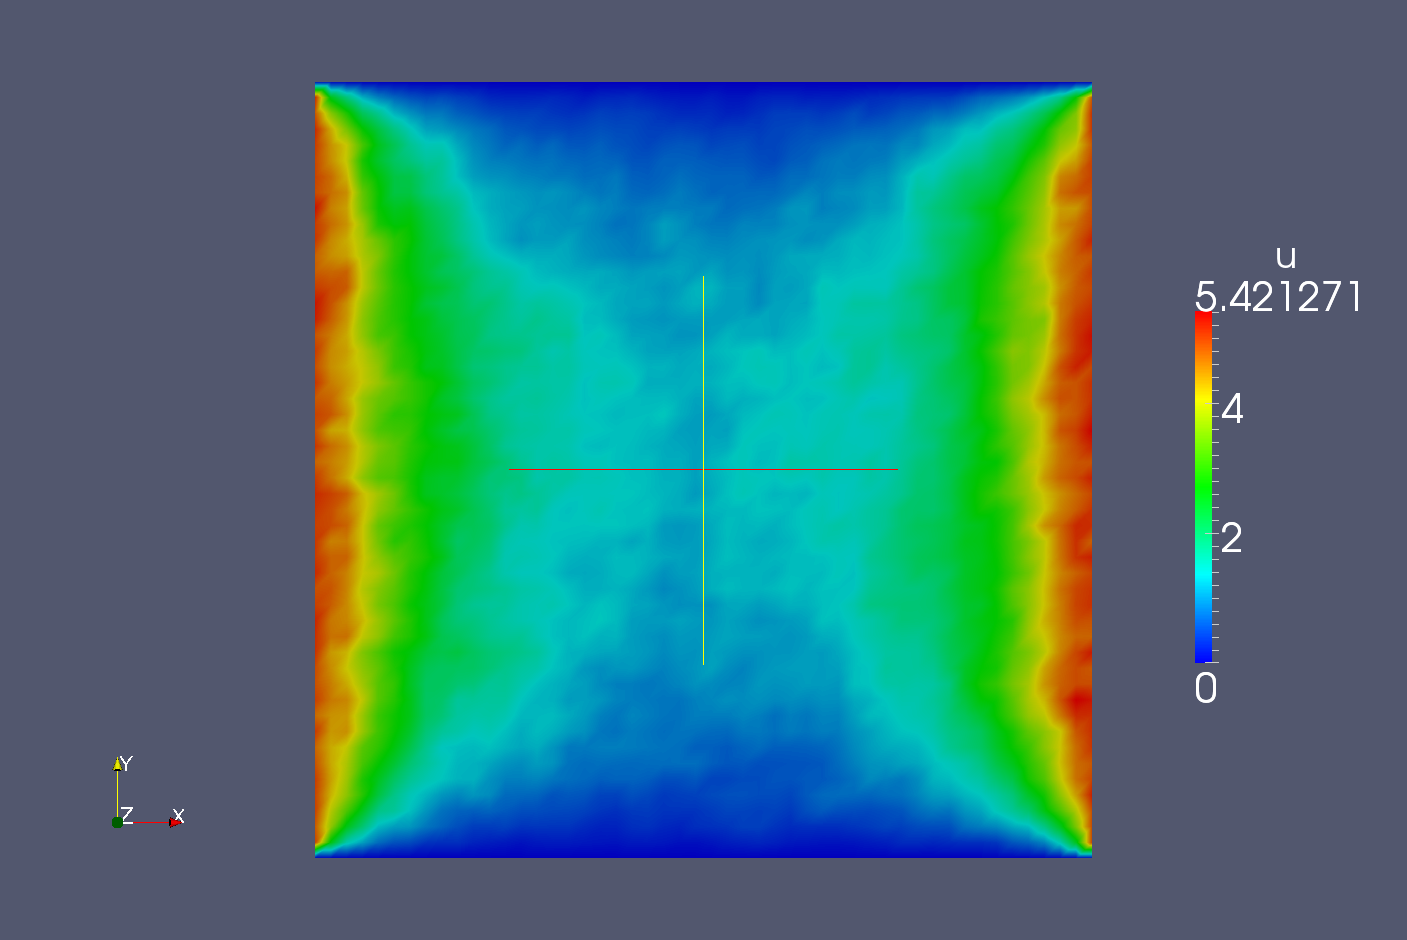
\includegraphics[width=4in]{adjoint_100000.png}
    \end{center}
    \caption{\textbf{Adjoint solution to Poisson Equation.}
      \textit{\sn{1}{5} total histories, 1.76 seconds CPU time.} }
  \end{figure}

\end{frame}

%%---------------------------------------------------------------------------%%
\begin{frame}{Adjoint Method: Evolution of a Solution}

  \begin{figure}[h!]
    \begin{center}
      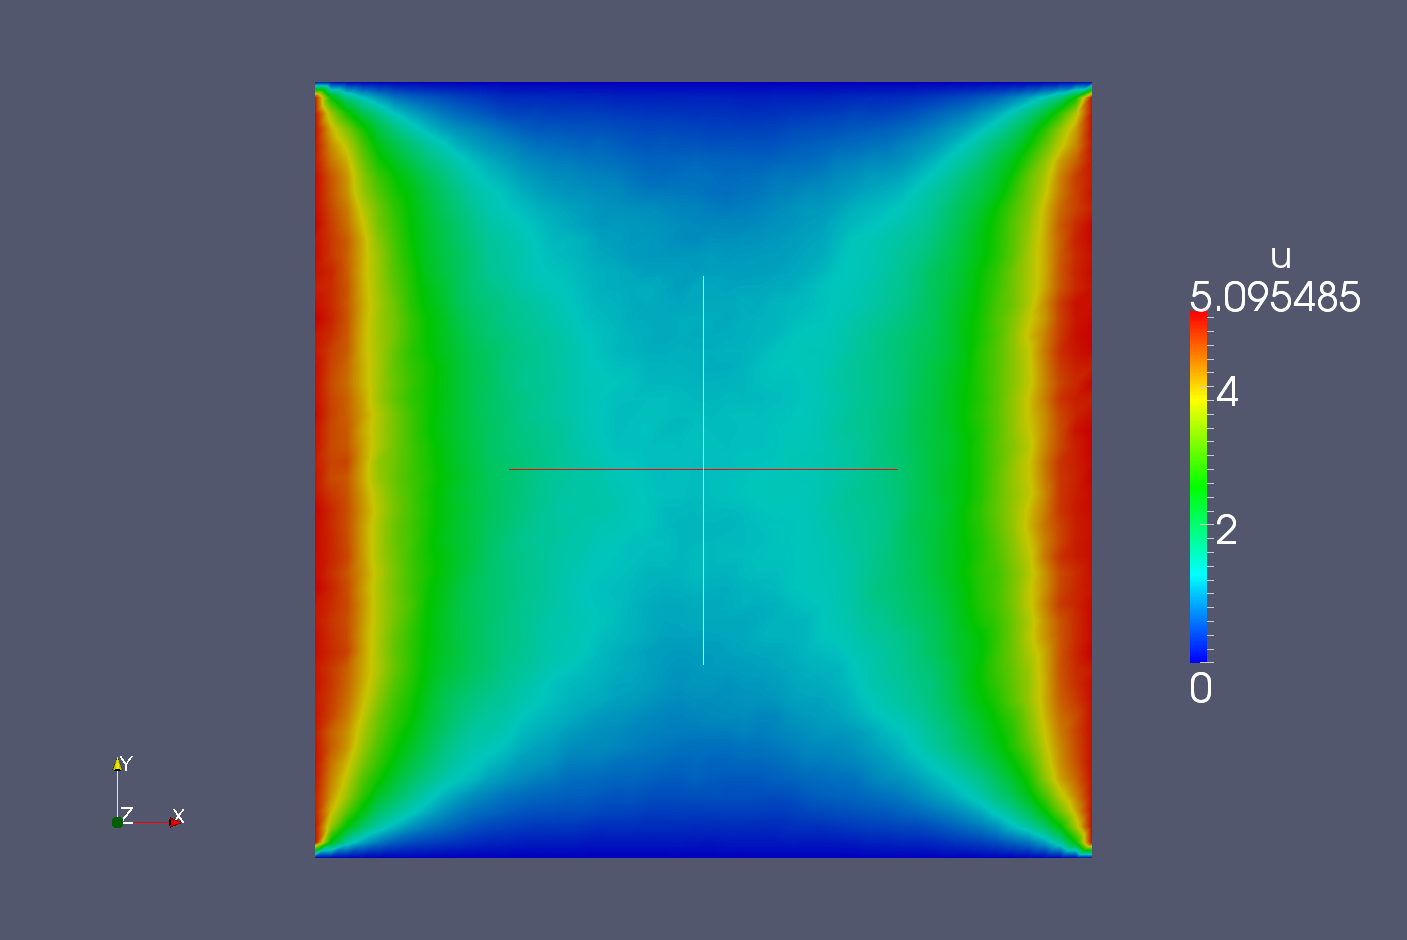
\includegraphics[width=4in]{adjoint_1000000.png}
    \end{center}
    \caption{\textbf{Adjoint solution to Poisson Equation.}
      \textit{\sn{1}{6} total histories, 15.1 seconds CPU time.} }
  \end{figure}

\end{frame}

%%---------------------------------------------------------------------------%%
\begin{frame}{Adjoint Method: Evolution of a Solution}

  \begin{figure}[h!]
    \begin{center}
      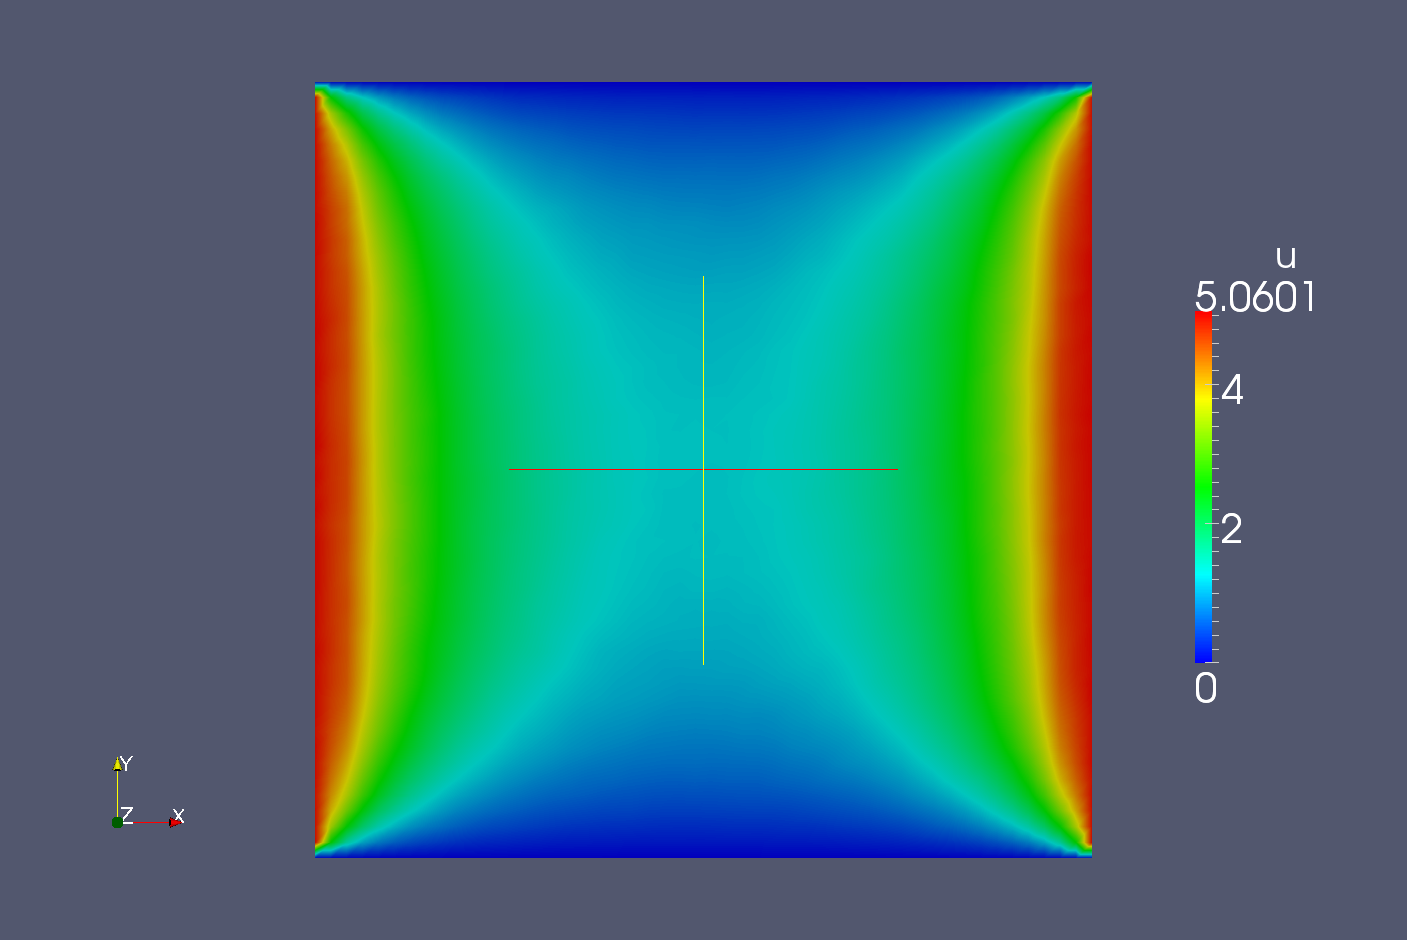
\includegraphics[width=4in]{adjoint_10000000.png}
    \end{center}
    \caption{\textbf{Adjoint solution to Poisson Equation.}
      \textit{\sn{1}{7} total histories, 149 seconds CPU time.} }
  \end{figure}

\end{frame}


%%---------------------------------------------------------------------------%%
\begin{frame}{Domain Decomposed Monte Carlo}

  \begin{columns}
    \begin{column}{0.5\textwidth}
      \begin{itemize}
      \item Each parallel process owns a piece of the domain (linear
        system)
        \bigskip
      \item Random walks must be transported between adjacent domains
        through parallel communication
        \bigskip
      \item Domain decomposition determined by the input system
      \end{itemize}
    \end{column}

    \begin{column}{0.5\textwidth}
      \begin{figure}[htpb!]
        \begin{center}
          \scalebox{0.75}{ \input{msod_example.pdftex_t} }
        \end{center}
        \caption{\textbf{Domain decompostion example illustrating how
            domain-to-domain transport creates communication costs.}}
      \end{figure}
    \end{column}
  \end{columns}

\end{frame}

%%---------------------------------------------------------------------------%%
\begin{frame}{Model Problem - 2D Neutron Diffusion}

  \begin{columns}

    \begin{column}{0.5\textwidth}
      \begin{figure}[t!]
        \begin{center}
          \scalebox{0.5}{\input{stencil.pdftex_t}}
        \end{center}
        \caption{\textbf{Nine-point Laplacian stencil.}}
      \end{figure}
    \end{column}

    \begin{column}{0.5\textwidth}
      \[
        -D \boldsymbol{\nabla}^2 \phi + \Sigma_a \phi = S
      \]

      \[
        \ve{D}\boldsymbol{\phi}=\ve{s}
      \]
    \end{column}

  \end{columns}

  \begin{multline}
    -\frac{1}{6h^2}[4 \phi_{i-1,j} + 4 \phi_{i+1,j} + 4 \phi_{i,j-1} + 4
      \phi_{i,j+1} + \phi_{i-1,j-1}\\ + \phi_{i-1,j+1} + \phi_{i+1,j-1}
      + \phi_{i+1,j+1} - 20 \phi_{i,j}] + \Sigma_a \phi_{i,j} = s_{i,j}
  \end{multline}

\end{frame}

%%---------------------------------------------------------------------------%%
\begin{frame}{Eigenvalue Computation}

\[
  \Phi_{p,q}(x,y) = e^{2 \pi \imath p x} e^{2 \pi \imath q y}
\]

\begin{multline}
  \ve{D}\Phi_{p,q}(x,y) = \lambda_{p,q}(\ve{D})
  =\\ -\frac{D}{6h^2}\Big[4 e^{-2 \pi \imath p h} + 4 e^{2 \pi \imath
      p h} + 4 e^{-2 \pi \imath q h} + 4 e^{2 \pi \imath q h} + e^{-2
      \pi \imath p h} e^{-2 \pi \imath q h} \\ + e^{-2 \pi \imath p h}
    e^{2 \pi \imath q h} + e^{2 \pi \imath p h} e^{-2 \pi \imath q h}
    + e^{2 \pi \imath p h} e^{2 \pi \imath q h} - 20\Big] + \Sigma_a
\end{multline}

\[
  \lambda_{p,q}(\ve{D}) = -\frac{D}{6h^2}[ 8 \cos(\pi p h) + 8
    \cos(\pi q h) + 4 \cos(\pi p h) \cos(\pi q h) - 20] + \Sigma_a
\]

\end{frame}

%%---------------------------------------------------------------------------%%
\begin{frame}{Jacobi Preconditioned Iteration Matrix Spectrum}

  \begin{columns}

    \begin{column}{0.5\textwidth}
      \begin{figure}[t!]
        \begin{center}
          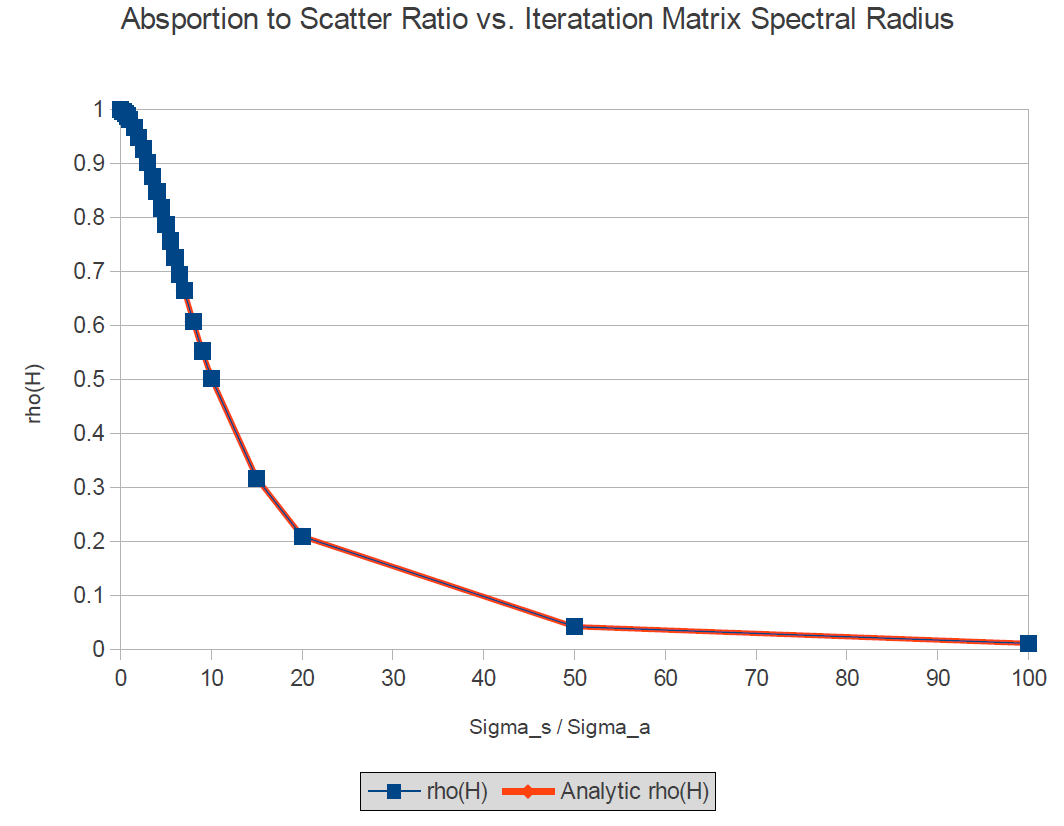
\includegraphics[width=2.5in,clip]{measured_spec_rad.png}
        \end{center}
        \caption{\textbf{Measured and analytic preconditioned diffusion
            operator spectral radius as a function of the absorption cross
            section to scattering cross section ratio.}}
      \end{figure}
    \end{column}

    \begin{column}{0.5\textwidth}
      \[
        \ve{M}^{-1} \ve{D} \boldsymbol{\phi} = \ve{M}^{-1} \ve{s}
      \]
      \medskip
      \[
        \lambda_{p,q}(\ve{M}^{-1} \ve{D}) = \alpha \lambda_{p,q}(\ve{D})
      \]
      \medskip
      \[
        \ve{H} = \ve{I} - \ve{M}^{-1} \ve{D}
      \]
      \medskip
      \[
        \rho(\ve{H}) = \frac{10 \alpha D}{3 h^2}
      \]
    \end{column}

  \end{columns}

\end{frame}

%%---------------------------------------------------------------------------%%
\begin{frame}{Random Walk Length}

  \[
  \ve{e}^{k} = \ve{H}^k\ve{e}^0 \ \ \rightarrow \ \ ||\ve{e}^{k}||_2
  \leq \rho(\ve{H})^k ||\ve{e}^0||_2 \ \ \rightarrow \ \ k \approx
  \frac{ \log(W_c) }{ \log( \rho(\ve{H}) ) }
  \]

  \bigskip
  \begin{figure}[t!]
    \begin{center}
      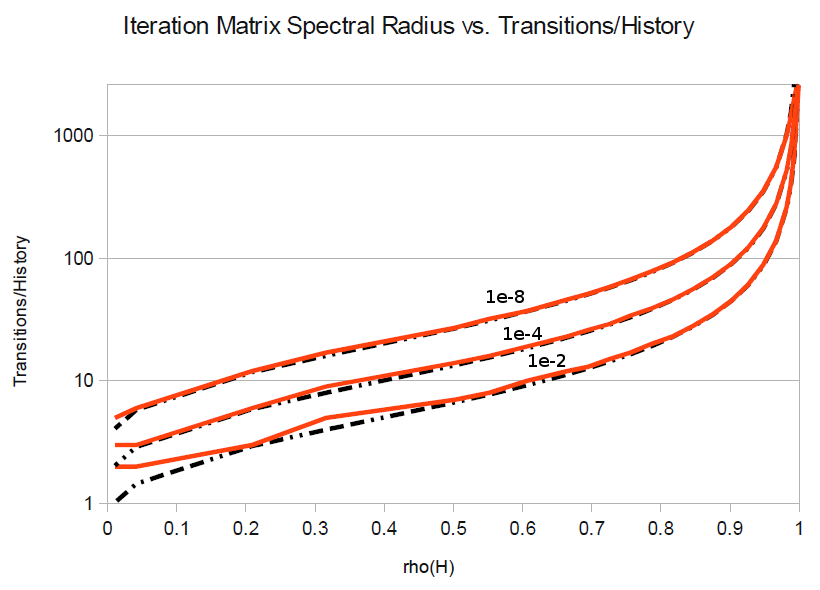
\includegraphics[width=4.5in,clip]{measured_length.png}
    \end{center}
    \caption{\textbf{Measured and analytic random walk length as a
        function of the iteration matrix spectral radius.}}
  \end{figure}

\end{frame}

%%---------------------------------------------------------------------------%%
\begin{frame}{Linear Operator Domain Optical Thickness}

  \begin{columns}

    \begin{column}{0.5\textwidth}

      \begin{itemize}
      \item $l$ = chord length
        \bigskip
      \item $n_i$ = \# of discrete states along the chord
        \bigskip
      \item $n_s$ = \# of discrete states per transition along the chord
        \bigskip
      \item $d$ = dimensionality of problem
      \end{itemize}

    \end{column}

    \begin{column}{0.5\textwidth}

      \[
      \langle \bar{r_1^2} \rangle = (n_s h)^2 \ \ \ \rightarrow
      \ \ \ \langle \bar{r_k^2} \rangle = k (n_s h)^2
      \]

      \[
      \langle \bar{r_k^2} \rangle = k \Bigg(\frac{n_s l}{n_i}\Bigg)^2
      \]

      \[
      \tau = \frac{l}{2 d \sqrt{\langle \bar{r_k^2} \rangle}}
      \]

      \[
      \tau = \frac{n_i}{2 d n_s \sqrt{k}}
      \]

      \[
      \tau = \frac{n_i}{2 d n_s}
      \sqrt{\frac{\log(\rho(\ve{H}))}{\log(W_c)}}
      \]

    \end{column}


  \end{columns}

\end{frame}

%%---------------------------------------------------------------------------%%
\begin{frame}{Choosing $n_i$ and $n_s$}

  \begin{columns}

    \begin{column}{0.5\textwidth}
      \begin{figure}[t!]
        \begin{center}
          \scalebox{0.5}{\input{stencil.pdftex_t}}
        \end{center}
        \caption{\textbf{Nine-point Laplacian stencil.}}
      \end{figure}
    \end{column}

    \begin{column}{0.5\textwidth}
      \[
      n_i = 5
      \]

      \[
      n_s = \frac{3}{5}
      \]
    \end{column}

  \end{columns}

  \begin{multline}
    -\frac{1}{6h^2}[4 \phi_{i-1,j} + 4 \phi_{i+1,j} + 4 \phi_{i,j-1} + 4
      \phi_{i,j+1} + \phi_{i-1,j-1}\\ + \phi_{i-1,j+1} + \phi_{i+1,j-1}
      + \phi_{i+1,j+1} - 20 \phi_{i,j}] + \Sigma_a \phi_{i,j} = s_{i,j}
  \end{multline}

\end{frame}

%%---------------------------------------------------------------------------%%
\begin{frame}{Domain Leakage Approximations}

  \[
    \Lambda = \frac{average\ \#\ of\ histories\ leaving\ local\ domain}
            {total\ of\ \#\ of\ histories\ starting\ in\ local\ domain}
  \]
  \bigskip

  \begin{beamerboxesrounded}[upper=boxheadcolor,lower=boxbodycolor,shadow=true]
    {Wigner Rational Approximation}
  \[
    \Lambda = \frac{1}{1+\tau}
  \]
  \end{beamerboxesrounded}
  \bigskip

  \begin{beamerboxesrounded}[upper=boxheadcolor,lower=boxbodycolor,shadow=true]
    {Mean Chord Approximation}
  \[
    \Lambda = \frac{1-e^{-\tau}}{\tau}
  \]
  \end{beamerboxesrounded}

\end{frame}

%%---------------------------------------------------------------------------%%
\begin{frame}{Domain Leakage Results}

  \begin{figure}[t!]
    \begin{center}
      \includegraphics[width=3.5in,clip]{leakage_variation.png}
    \end{center}
    \caption{\textbf{Measured and analytic domain leakage as a
        function of the iteration matrix spectral radius.} The red
      data was computed numerically by a domain-decomposed adjoint
      Neumann-Ulam implementation, the black dashed data was generated
      using the mean-chord approximation, and the dashed-dotted black
      data was generated using the Wigner rational approximation.}
  \end{figure}

\end{frame}

%%---------------------------------------------------------------------------%%
\begin{frame}{Domain Leakage Results}

  \begin{figure}[ht!]
      \begin{center}
        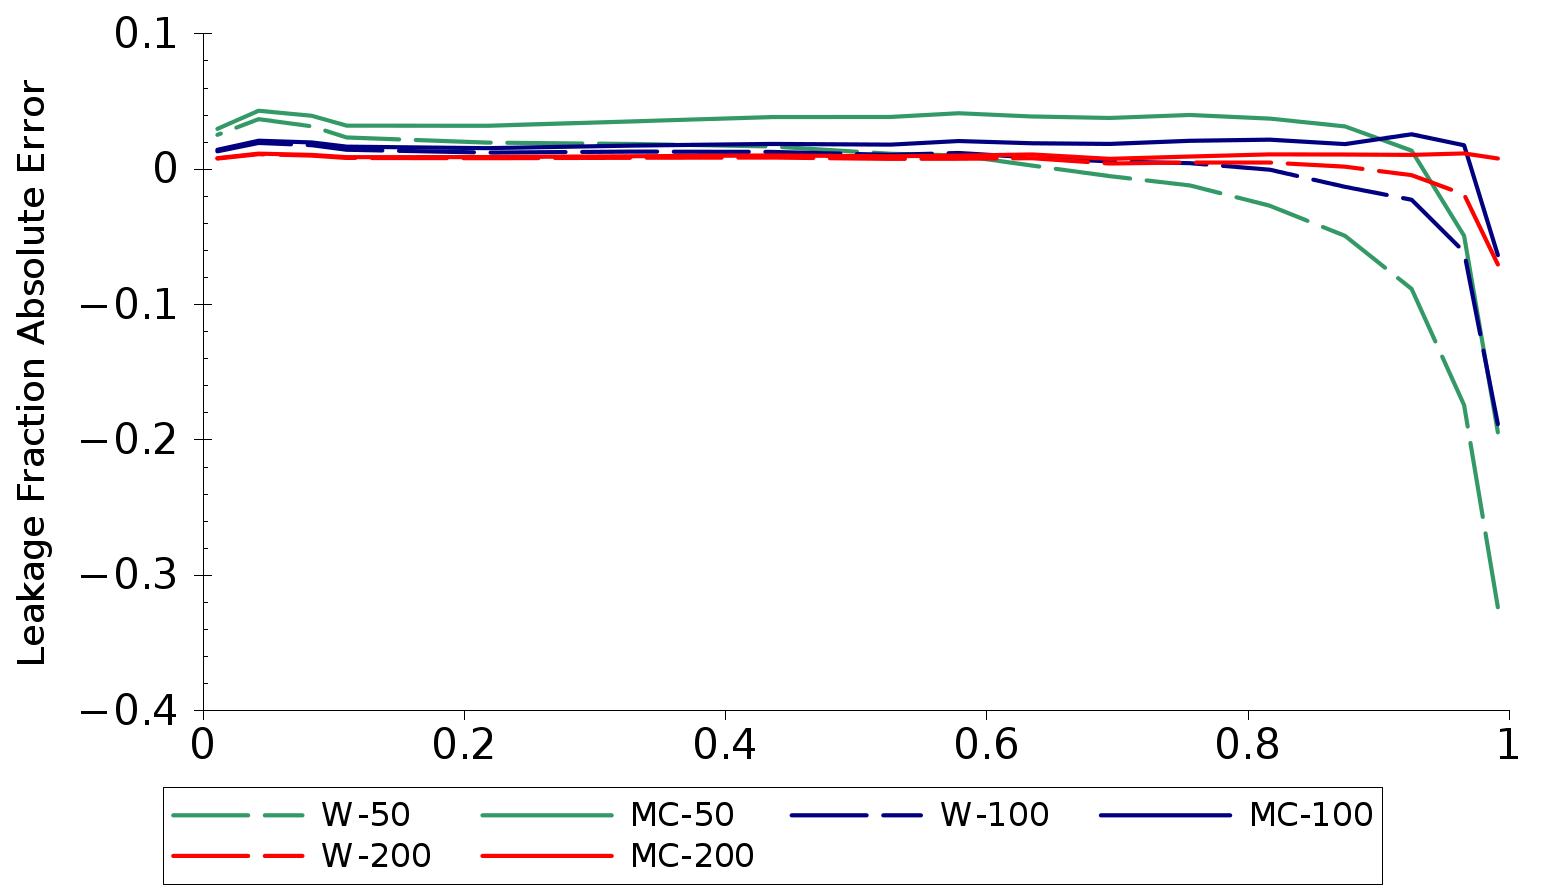
\includegraphics[width=4.0in,clip]{leakage_error.png}
      \end{center}
      \caption{\textbf{Measured and analytic domain leakage absolute
          error as a function of the iteration matrix spectral radius.}}
  \end{figure}

\end{frame}

%%---------------------------------------------------------------------------%%
\begin{frame}{Conclusions and Future Work}

  \begin{itemize}
  \item Good agreement between theory and numerical experiments
    \bigskip
  \item Extension to asymmetric systems and communcation cost analysis
    \bigskip
  \item Coordinate measurements with massively parallel computations
    \bigskip
  \item Explore in the context of synthetic acceleration methods
  \end{itemize}

\end{frame}

%%---------------------------------------------------------------------------%%
\begin{frame}{Acknowledgements}

This work was performed under appointment to the Nuclear Regulatory
Commission Fellowship program at the University of Wisconsin - Madison
Engineering Physics Department.

\end{frame}

%%---------------------------------------------------------------------------%%

\end{document}
